% Section 5 (group B): Koide as geometry. Sources: Companion thm:koide-triolic (status), rounds v4.10.0-r12, r13.2, r14,
% r15, r16, r17, r19, r25, r28, r30, r31 (H118), r59; tests from wiki/Vorhersagen-und-Tests.md.
\section{Koide as geometry, not as derivation}
\label{sec:B-koide}

For three non-negative mass roots $x_k=\sqrt{m_k}$ the Koide ratio is
\begin{equation}
 K=\frac{\sum_k x_k^2}{\bigl(\sum_k x_k\bigr)^2}\in\bigl[\tfrac13,1\bigr].
 \label{eq:B-koide}
\end{equation}
For the charged-lepton pole masses $K=\tfrac23$ holds to better than $0.005\,\%$ \cite{Koide1983}. In the Companion this is an
empirical fact whose derivation is \Open{} (\cite{QSC}, \texttt{thm:koide-triolic}; \rnd{r12}.1). This section collects
what the construction says about it. The result is geometric and largely \Established: $K=\tfrac23$ is equivalent to a
statement about three states with overlap $\tfrac12$, the boundary of the admissible family is the octant of a qubit, and the
bend away from the boundary has an exact form. None of it derives $K=\tfrac23$.

We state the point plainly, because it is easy to miss in a calculation. \emph{The overlap $\tfrac12$ is an input.} Every
construction below that produces $K=\tfrac23$ does so because the overlap $\tfrac12$, or a parameter condition equivalent to
it, was put in. Inserting such a condition (the radius $r=\sqrt2$ of the Brannen form, equal weights of two couplings, or any
fixed ratio of parameters chosen to give $\rho^2=\tfrac12$) presupposes the Koide relation; it does not explain it.

\subsection{The Gram reading}
\label{sec:B-gram}

Let $v_1,v_2,v_3$ be unit vectors with Gram matrix $G_{ij}=\langle v_i,v_j\rangle$, and read the mass roots as the eigenvalues
of $G$ up to a common scale, $x_k=s\,\lambda_k(G)$. This root law is itself a setting.

\begin{proposition}[\rnd{r12}.2]\label{prop:B-gram}
Put $\rho^2=\tfrac13\sum_{i<j}|\langle v_i,v_j\rangle|^2$. Then
\begin{equation}
 K=\frac{\operatorname{Tr}G^2}{(\operatorname{Tr}G)^2}=\frac{1+2\rho^2}{3},\qquad
 K=\tfrac23\iff\rho^2=\tfrac12 .
 \label{eq:B-K-rho}
\end{equation}
\end{proposition}

\begin{proof}
$\operatorname{Tr}G=3$ and $\operatorname{Tr}G^2=\sum_{ij}|G_{ij}|^2=3+2\sum_{i<j}|G_{ij}|^2=3+6\rho^2$. Since $G$ is Hermitian
and positive semidefinite, $\sum_k\lambda_k^2=\operatorname{Tr}G^2$ and $\sum_k\lambda_k=\operatorname{Tr}G$.
\end{proof}

Thus $K=\tfrac23$ is a mean squared overlap of $\tfrac12$: three readout states pairwise half-way, in Fubini--Study distance
$\pi/4$, between equal and orthogonal. Equivalent forms are on record: the angle $\pi/4$ between the root vector and
$(1,1,1)$ \cite{Foot1994}, and the Brannen parametrisation $x_k=a[1+r\cos(\theta+2\pi k/3)]$ with $K=\tfrac13+r^2/6$, so
$K=\tfrac23\iff r=\sqrt2$ \cite{Brannen2010}. The remark that ``$\tfrac23$ is everywhere'' in the construction is a list
of coincidences and not a result (\rnd{r12}.2).

\subsection{The bent octant}
\label{sec:B-bent}

Fix the three pairwise overlaps at $|G_{ij}|^2=\tfrac12$. Rephasing $v_j\mapsto e^{i\alpha_j}v_j$ changes $G_{ij}$ by
$e^{i(\alpha_j-\alpha_i)}$ and leaves the Bargmann invariant $G_{12}G_{23}G_{31}=e^{i\varphi}/(2\sqrt2)$ unchanged, so the
triple is characterised by one phase $\varphi$. A convenient representative is circulant,
\begin{equation}
 G(\varphi)=I_3+\tfrac1{\sqrt2}\bigl(e^{i\varphi/3}U+e^{-i\varphi/3}U^*\bigr),\qquad U(z_1,z_2,z_3)=(z_2,z_3,z_1),
 \label{eq:B-circulant}
\end{equation}
with eigenvalues
\begin{equation}
 \lambda_k(\varphi)=1+\sqrt2\cos\Bigl(\frac{\varphi}{3}+\frac{2\pi k}{3}\Bigr),\qquad k=0,1,2,
 \label{eq:B-roots}
\end{equation}
which is the Brannen form at $r=\sqrt2$ with $\theta=\varphi/3$.

\begin{proposition}[Bent axes, \rnd{r14}.5]\label{prop:B-bent}
Three states with pairwise overlap $\tfrac12$ give $K=\tfrac23$ for every Bargmann phase $\varphi$, and
\begin{equation}
 \det G=\tfrac12\bigl(\sqrt2\cos\varphi-1\bigr).
 \label{eq:B-detG}
\end{equation}
In the principal range, $G$ is positive definite for $|\varphi|<\pi/4$ (three positive roots, the states span
$\mathbb C^3$), has rank two at $|\varphi|=\pi/4$ (one root vanishes, the states lie in one qubit), and is not a Gram
matrix for $|\varphi|>\pi/4$.
\end{proposition}

\begin{proof}
$K=\tfrac23$ follows from Proposition~\ref{prop:B-gram}. For a $3\times3$ matrix with unit diagonal,
$\det G=1-\sum_{i<j}|G_{ij}|^2+2\operatorname{Re}(G_{12}G_{23}G_{31})=1-\tfrac32+\tfrac{1}{\sqrt2}\cos\varphi$. All
$2\times2$ principal minors equal $\tfrac12>0$, so by Sylvester's criterion positivity is decided by the sign of $\det G$.
\end{proof}

The formula and its zero at $\varphi=\pi/4$ are checked numerically against the circulant matrix (deviation below
$10^{-15}$, script \texttt{F6\_detG.py}); Figure~\ref{fig:B-detG} shows both.

\paragraph{The flat octant is the boundary.}
For a qubit, $|\langle a|b\rangle|^2=\tfrac12(1+\mathbf n_a\cdot\mathbf n_b)$ with Bloch vectors $\mathbf n$. Overlap $\tfrac12$
therefore means orthogonal Bloch vectors, and three qubit states with pairwise overlap $\tfrac12$ are, up to rotation, the
eigenstates $+x,+y,+z$ of $\sigma_x,\sigma_y,\sigma_z$: the octant. Its geodesic triangle encloses the solid angle $\pi/2$,
and its Bargmann phase is half of it, $\pi/4$. The octant is rigid: on the Bloch sphere a smaller enclosed area with the
same overlaps is impossible, and the states always have rank two. Hence the boundary of the Koide arc,
$\rho^2=\tfrac12$ at $\varphi=\pi/4$, is exactly the octant triple of three spin-$\tfrac12$ states (\rnd{r12}.4(c)),
with roots $\bigl(\tfrac{3+\sqrt3}{2},0,\tfrac{3-\sqrt3}{2}\bigr)$: one mass is zero. \Established.

\paragraph{Bending needs a third dimension.}
Three positive masses require $\varphi<\pi/4$ and hence leave the qubit for $\mathbb C^3$. The charged-lepton root ratios
$1:14.38:58.97$ are reproduced at $\varphi=\tfrac23$ (Brannen's $\delta=\tfrac29$ times three), with $\det G=0.0557$; this
value is fitted, not derived, and the bend $\pi/4-\tfrac23=0.118731$ is the quantity to be explained. One native way to leave the
qubit is spin one (\rnd{r15}.3): three spin-1 coherent states, symmetric about a cycle axis, with pairwise overlap
$\cos^4(a/2)=\tfrac12$ have side angle $\cos a=\sqrt2-1$, axis angle $38.68^\circ$, $K=\tfrac23$ and Bargmann phase
\begin{equation}
 \varphi=3\arccos\bigl(1-\tfrac1{\sqrt2}\bigr)-\pi=0.679042,\qquad \det G=0.0503,
 \label{eq:B-spin1}
\end{equation}
rank three with root ratios $1:16.24:65.93$. Spin-$j$ coherent-state overlaps are the $2j$-th powers of the spin-$\tfrac12$
overlaps, so the Bargmann phase is $j$ times the enclosed solid angle (a standard property \cite{Perelomov1986}, not a Companion
result); the spin-one triangle is smaller than the octant and bends without any extra structure. The remainder to the lepton
phase is $0.012376$, and no native axis was found among 143 candidates fixed beforehand. The direction is not independent: it
follows from the overlap $\tfrac12$ alone. Symmetric constructions on the carrier fix $\varphi$ by their spin
($0.785$, $0.679$, $0.650$, $0.637$ for $j=\tfrac12,1,\tfrac32,2$), and $\tfrac23$ is not among them (\rnd{r28}.2).
Figure~\ref{fig:B-bloch} shows the flat octant and the spin-one triangle.

\begin{figure}[t]
\centering
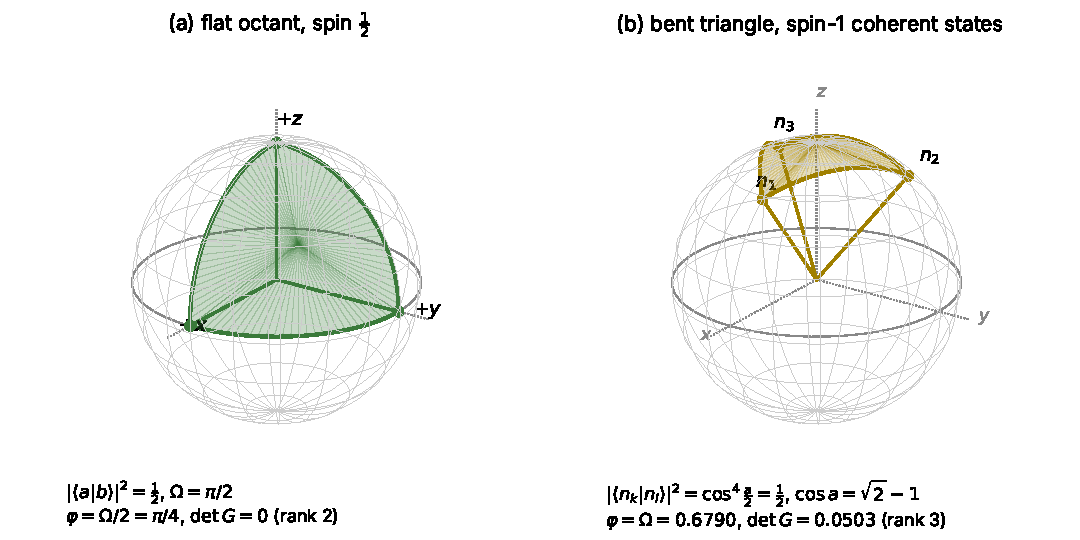
\includegraphics[width=\textwidth]{figures/F5-koide-bloch.pdf}
\caption{Flat against bent. (a) Three spin-$\tfrac12$ states with pairwise overlap $\tfrac12$ have orthogonal Bloch vectors:
the octant, solid angle $\pi/2$, Bargmann phase $\pi/4$, $\det G=0$, one mass zero (\rnd{r12}.4(c), \rnd{r14}.5).
(b) Directions of three spin-1 coherent states with the same overlap: side angle $\cos a=\sqrt2-1$, solid angle and phase
$0.679042$, $\det G=0.0503$, three positive masses (\rnd{r15}.3). Both panels have $K=\tfrac23$ because the overlap
$\tfrac12$ is put in. Status: exact geometry; the physical readout is a setting. Numbers from \texttt{scripts/F5\_koide\_bloch.py}.}
\label{fig:B-bloch}
\end{figure}

\begin{figure}[t]
\centering
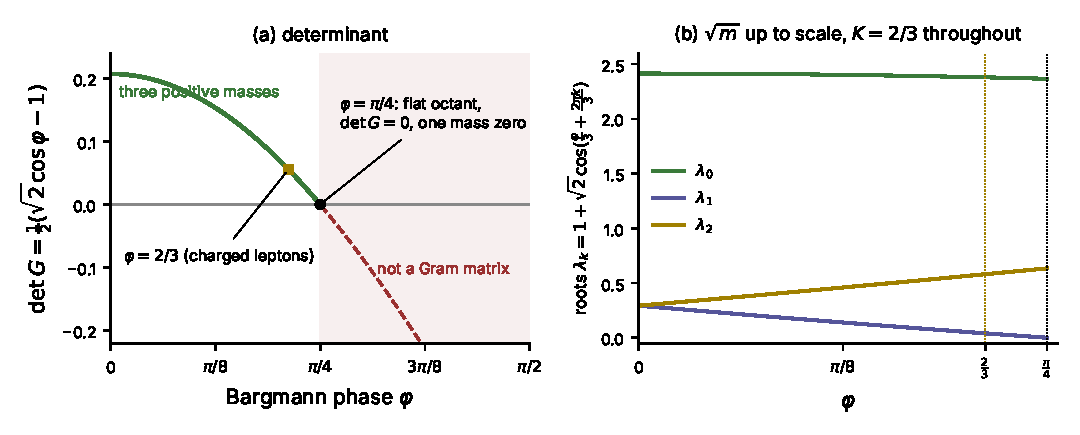
\includegraphics[width=\textwidth]{figures/F6-detG.pdf}
\caption{(a) $\det G=\tfrac12(\sqrt2\cos\varphi-1)$ for three states with pairwise overlap $\tfrac12$. It vanishes exactly at
$\varphi=\pi/4$ (flat octant, one massless state) and is negative beyond, where no Gram matrix exists. The square marks
$\varphi=\tfrac23$, where the circulant roots reproduce the charged-lepton ratios (a fit). (b) The three roots
\eqref{eq:B-roots}; $K=\tfrac23$ on the whole interval. Status: exact (\rnd{r14}.5); the value of $\varphi$ is not derived.
Numbers from \texttt{scripts/F6\_detG.py}.}
\label{fig:B-detG}
\end{figure}

\paragraph{A guarded core as reading.}
The Companion offers one reading of the bend, recorded as a \Reading{} (\rnd{r14}.6). Read a flux-free cap of solid angle
$\Omega$ on the generation sphere (the guarded core of the orbit scan) as removed from the octant. On a sphere with $n$ caps
there are $n-1$ free Aharonov--Bohm holonomies; exactly one core is the only number that bends without a free parameter. If
the displaced flux sits at the antipode, which the antilinear reflector with $\Theta^2=-1$ suggests, the phase is
$\varphi=\pi/4-\Omega/2$. With $\Omega=\gamma_M=0.237533$, the matter-frame value of Section~\ref{sec:beta}, this is the relation of test
H102, $m_\tau=1777.134$\,MeV (exact Koide gives $1776.969$\,MeV). H102 rests on the placeholders CT-001 and CT-002; it is
\Open{} until the first PDG edition after 13~November 2026 (at the latest end of 2028), and against PDG 2024
($1776.93\pm0.09$\,MeV, unchanged in PDG 2026) it stands at $+2.3\sigma$ (\rnd{r28}.3). The core size is thereby OP1 again
(\rnd{r14}.7, \rnd{r28}.2).

\subsection{Why three, and why one half: complementarity}
\label{sec:B-complementarity}

The octant consists of one eigenstate each of $\sigma_x$, $\sigma_y$, $\sigma_z$, one state from each of the three mutually
unbiased bases of a qubit. This generalises.

\begin{proposition}[\rnd{r15}.4]\label{prop:B-mub}
In dimension $d$ take one state from each of $d+1$ mutually unbiased bases. The $N=d+1$ states have
\begin{equation}
 K=\frac{\operatorname{Tr}G^2}{(\operatorname{Tr}G)^2}=\frac{2}{d+1}=\frac2N ,
 \label{eq:B-mub}
\end{equation}
and their Gram matrix has rank at most $d<N$. Only $d=2$ gives three states, with $K=\tfrac23$.
\end{proposition}

\begin{proof}
States from different unbiased bases have overlap $1/d$. Hence $\operatorname{Tr}G=N$ and
$\operatorname{Tr}G^2=N+N(N-1)/d=2N$, because $N-1=d$. The rank bound holds because the states lie in $\mathbb C^d$.
\end{proof}

Read this way, ``three generations'' and ``Koide $\tfrac23$'' are one statement, $K=2/N$ at $N=3$. Two principles are assumed:
one state per complementary basis, and a complete set. \Reading.

\subsection{The octant on a Lorentz-invariant doublet}
\label{sec:B-doublet}

Where could three such states live natively? Round \rnd{r16} places them on the field doublet. With $F_\pm=E\pm iB$ and the
bilinear squares $s_\pm=F_\pm\cdot F_\pm$, a boost acts on $F_+$ by some $M\in SO(3,\mathbb C)$ and on $F_-$ by $\bar M$, so
$s_\pm$ are invariant and
\begin{equation}
 \chi=\bigl(\sqrt{s_+},\sqrt{s_-}\bigr)
 \label{eq:B-chi}
\end{equation}
is a doublet whose Bloch sphere does not depend on the observer. Real fields lie on its equator, self-dual and anti-self-dual
non-null fields at the poles, and plane waves ($s_+=s_-=0$) have no point. The roots carry a sign; a point of $\chi$ is fixed
up to $R$. On $\chi$ the three frame maps of Section~\ref{sec:A-frames} act, up to phase, as
\begin{equation}
 R=\sigma_z,\qquad T=\sigma_x,\qquad J_B=\sigma_y
 \label{eq:B-frame-pauli}
\end{equation}
(checked on 200 real fields, deviation $4\cdot10^{-16}$). Each keeps exactly one of three field signs, $R$ the helicity sign,
$T$ the sign of $\operatorname{Re}s$ (matter against tachyon), $J_B$ the sign of $\operatorname{Im}s$; on the signs they form
the Klein four-group. A matter field ($s=1$), a field of the photon side ($s=i$) and a self-dual field ($E=iB$) give pairwise
overlap $\tfrac12$, $K=\tfrac23$ and Bargmann phase $\pm\pi/4$, and all three rays are unchanged under boosts (\rnd{r16}.3).
The phase needs complex amplitudes: for every octant $\sum_kb_{y,k}^2=1$ in the helicity component, and three states without
helicity component have phase $0$ or $\pi$ (\rnd{r16}.2). The three bases of the doublet, their Stokes-type sphere and the
helicity axis are in the literature \cite{A-Golat2024}; in the Companion's language they are the eigenbases of $T$, $J_B$ and $R$.

\begin{proposition}[Readouts of one object, \rnd{r16}.7]\label{prop:B-readouts}
The eigenrays of $R$, $T$, $J_B$ on $\chi$ are the six poles $\pm x,\pm y,\pm z$. A set of these poles without an
orthogonal pair has at most three elements; there are exactly eight such sets of three, and each is an octant with pairwise
overlap $\tfrac12$, $K=\tfrac23$ and Bargmann phase $\pm\pi/4$.
\end{proposition}

\begin{proof}
Two poles are orthogonal exactly when they are antipodal. A set without an antipodal pair contains at most one pole from each
of the three axes, so at most three elements, and the maximal sets are the $2^3=8$ choices of one sign per axis. Poles from
different axes have orthogonal Bloch vectors and overlap $\tfrac12$; the rest is the octant computation above.
\end{proof}

The reading attached to this is \Reading{} and \emph{not blind}: require (1) that a readout is an eigenstate of a frame map,
(2) that two readouts of one object are not orthogonal, and (3) that all such readouts occur. Then the number three, the overlap
$\tfrac12$ and the phase $\pi/4$ follow together, unique up to frame maps and orientation, and no threefold cycle is needed.
The targets were known and the conditions were stated afterwards; (1), (3), the sign of the phase, the bend and a charged
carrier remain open. The last point is serious: by Proposition~\ref{prop:B-commutant} the generation index cannot sit on the
frame doublet of one generation, so on a charged carrier this reading takes the number of generations as input (\rnd{r19}.2).
The computations on the field doublet stand.

\paragraph{Prior art.}
The octant triple from three mutually unbiased bases, its phase $e^{i\pi/4}$, amplitudes as roots of $z^3=(1+i)/4$, the
charged-lepton form $1+\sqrt2\cos(2g\pi/3+2/9)$ and the neutrino phase $2/9+\pi/12$ appear in Brannen \cite{Brannen2010};
the angle $\pi/4$ is due to Foot \cite{Foot1994}, and $\delta\approx2/9$ is discussed by \.Zenczykowski \cite{Zenczykowski2012}.
The octant, its phase and the shift $\pi/12$ are therefore not results of the Companion. What is specific here is their
placement on the frame maps of the field doublet, restricted by \rnd{r19}.2 (\rnd{r19}.4).

\subsection{The Brannen form as a time cycle}
\label{sec:B-time-cycle}

The doublet also carries a native threefold cycle. For time-harmonic fields the instantaneous invariant decomposes exactly as
\begin{equation}
 s(t)=\bigl(E(t)+iB(t)\bigr)^2=\tfrac14\bigl(s_+e^{-2i\omega t}+2w+\bar s_-e^{2i\omega t}\bigr),\qquad w=F_+\cdot\bar F_-,
 \label{eq:B-st}
\end{equation}
and $w$ is a third Lorentz invariant (\rnd{r16}.8). Translation by one third of the period of $s(t)$ acts on $(s_+,w,\bar s_-)$
as $U=\operatorname{diag}(\bar\omega_3,1,\omega_3)$, $\omega_3=e^{2\pi i/3}$. A state with weights $(p_-,p_0,p_+)$,
$\sum p=1$, has an orbit of three states with circulant Gram matrix and
\begin{equation}
 |\langle\psi|U\psi\rangle|^2=\bigl|p_0+p_-\bar\omega_3+p_+\omega_3\bigr|^2=\tfrac12\Bigl(3\sum_kp_k^2-1\Bigr),
 \label{eq:B-autocorr}
\end{equation}
so Koide is $\sum p^2=\tfrac23$, with $p_k=\sqrt{m_k}/\sum\sqrt m$: the autocorrelation of the invariant after one third of
its period has modulus $1/\sqrt2$ (\rnd{r16}.9). The cycle is native and produces the Brannen form; the weights are Brannen's
parameters in another form. No principle in the inventory fixes $\sum p^2=\tfrac23$, and a search over 24 candidate constants
listed beforehand found no hit. The photon-clock functional of the Companion has the same form, but no window threshold lies at
$\tfrac12$, so the clock does not fix the overlap either (\rnd{r17}.1). Reading the overlap $\tfrac12$ as maximal
uncertainty (a one-bit question with probability $\tfrac12$) is a further \Reading{} with the maximisation assumed
(\rnd{r17}.2). All of this is \Exploration, not blind.

\subsection{The orientation of the octant step}
\label{sec:B-koide-orientation}

The octant fixes the modulus of the phase, not its sign. The loops $x\to y\to z\to x$ and $x\to z\to y\to x$ have the same
endpoints and the same three transition probabilities $\tfrac12$, but ordered overlap products $(1+i)/4$ and its conjugate,
steps of $+\pi/4$ and $-\pi/4$. Three pre-registered tests, all \emph{not blind} because the outcome was fixed analytically
beforehand, locate the open choice (\rnd{r30}.10--.12):
\begin{itemize}
\item H115: on the closed odd generation states $JS=-S$, so the direct compensator gives $CS=0$, rank zero. A real rank-five
halving exists only with an additional phase choice on a complex null line.
\item H116: magnitudes and endpoints do not fix the sign; even a uniform histogram of accumulated phases says nothing, since
both constant step sequences $\pm1$ modulo eight visit all eight phases.
\item H117: in a two-window model, of the 16 mask pairs three give $+\pi/4$, three give $-\pi/4$, nine are blocked and one is
ambiguous; no repair rule decides between the signs.
\end{itemize}

Test H118 then classifies the sign (\rnd{r31}.1). For the eight triples of Proposition~\ref{prop:B-readouts} the Bargmann
phase is exactly
\begin{equation}
 \varphi=\tau\,\varepsilon\,\frac{\pi}{4},
 \label{eq:B-orientation}
\end{equation}
with $\tau=\pm1$ the direction of the loop $R\to T\to J_B$ and $\varepsilon$ the product of the three pole signs.
$R$, $T$, $J_B$ and parity ($E\mapsto-E$, acting as $\sigma_x$) preserve the orientation; time reversal of the complex field
amplitudes ($E\mapsto\bar E$, $B\mapsto-\bar B$) maps $s_\pm\mapsto\bar s_\pm$, acts on $\chi$ as complex conjugation and
reverses it. This is the distinction of Section~\ref{sec:A-frames}: time reversal $z\mapsto\bar z$ is not the tachyon map $z\mapsto iz$. None of
nine candidates listed beforehand selects an orbit natively. H118a (the formula) is confirmed, H118b (a native selection) is
\Refuted. The sign of the octant step is a time orientation of the readout and is not fixed by the Companion. Round
\rnd{r59} followed this handedness further and found it set at every step, ending at the choice of $i$, a convention; only the
relative sign between leptons and quarks of Section~\ref{sec:B-cp} is not a convention.

\subsection{Tests that ground the result}
\label{sec:B-koide-tests}

Table~\ref{tab:B-koide-tests} lists the tests that bear on this section. Two are open predictions. The refuted ones are
listed because they ground a negative result: the Bargmann phase is rigid in the carrier geometry. Copies, entanglement,
frame-dependent readouts and nested normalisations of the carrier states (H106--H111) do not move the phase from the
spin-one value $0.679$ to $\tfrac23$; only a change of the connection on the generation sphere, as in the core reading, escapes
this rigidity (\rnd{r28}.2).

\begin{table}[t]
\centering\small
\begin{tabularx}{\textwidth}{@{}l>{\raggedright\arraybackslash}X>{\raggedright\arraybackslash}p{0.27\textwidth}@{}}
\toprule
test & statement & status\\
\midrule
H99 & equal overlap $\rho^2=\tfrac12$ for charged leptons and neutrinos, $\theta_\nu=\theta_e+\pi/12$:
$\Delta m^2_{21}/\Delta m^2_{31}=0.030839$ & compatible, $+1.80\sigma$ (NuFIT 6.1); \emph{not blind} (\rnd{r12}.5)\\
H100 & three values of that ratio fixed for the next NuFIT release & open (\rnd{r12}.5)\\
H101 & lepton mask lifts the electron off the qubit octant & refuted: the form preserves the rank, the electron stays massless\\
H102 & $\varphi_e=\pi/4-\gamma_M/2$ gives $m_\tau=1777.134$\,MeV & open; $+2.3\sigma$ against PDG 2024 (\rnd{r28}.3)\\
H103a & inherited charge fixes the magic-angle reference on $N$ & refuted; gives $K=\tfrac12$ (\rnd{r13}.1)\\
H106--H111 & carrier variants (singlet admixture, nested normalisation, entangled copies, frame-dependent readouts, time octant)
close the residual bend & refuted; no hit (\rnd{r28})\\
H115--H117 & compensator, endpoints or two windows fix the sign of the octant step & as stated above; not blind (\rnd{r30})\\
H118 & a native structure fixes the orientation & formula confirmed, selection refuted (\rnd{r31})\\
\bottomrule
\end{tabularx}
\caption{Tests bearing on the Koide geometry (status from \texttt{wiki/Vorhersagen-und-Tests.md} and the cited rounds).}
\label{tab:B-koide-tests}
\end{table}

\paragraph{Summary of the section.}
\Established: $K=(1+2\rho^2)/3$; three states with overlap $\tfrac12$ give $K=\tfrac23$ for every phase, with
$\det G=\tfrac12(\sqrt2\cos\varphi-1)$; the boundary is the rigid qubit octant with one massless state; $K=2/(d+1)$ for
complete sets of unbiased states; on the invariant doublet $\chi$ the non-orthogonal frame eigenstates are at most three
and form exactly the octants; the sign of the step is a time orientation. \Reading: the complementarity reading, the
readouts of one object, the time cycle and the guarded core. \Open: the overlap $\tfrac12$ itself, the bend to
$\varphi=\tfrac23$ (equivalently the core size, OP1), the orientation, and a charged carrier with three generations. The
Koide relation is described, not derived; OP3 remains open.
